%这个是根据计算机学报官网下的LaTeX模板改的，主要修改内容：①把GBK编码改成了UTF-8编码。②引入zhwinfonts，用上传的字体文件实现了字体的使用。
%现存的问题：①中文无法使用加粗功能，但是英文可以。解决方式1：使用黑体来凑合代替。解决方式2：在PDF编辑器里面一个一个加粗。②无法实现模板中所要求的每页脚注从1开始的要求。
%如果您在使用该模板的过程中遇到问题，或者有对该模板的修改意见，请联系本人：微信PolarisRisingWar（诸神缄默不语），或者CSDN诸神缄默不语（PolarisRisingWar）

\documentclass[10.5pt,compsoc]{CjC}
\usepackage{CJKutf8}
% \usepackage{CJK}
% \usepackage{xeCJK}
\usepackage{graphicx}
\usepackage{footmisc}
\usepackage{subfigure}
\usepackage{url}
\usepackage{multirow}
\usepackage[noadjust]{cite}
\usepackage{amsmath,amsthm}
\usepackage{amssymb,amsfonts}
\usepackage{booktabs}
\usepackage{color}
\usepackage{ccaption}
\usepackage{booktabs}
\usepackage{float}
\usepackage{fancyhdr}
\usepackage{caption}
\usepackage{xcolor,stfloats}
\usepackage{comment}
\setcounter{page}{1}
\graphicspath{{figures/}}
\usepackage{cuted}%flushend,
\usepackage{captionhack}
\usepackage{epstopdf}
\usepackage[utf8]{inputenc}
%\usepackage{ccmap}
%\CJKtilde
%\usepackage{CJKpunct} 
%\usepackage[lite,subscriptcorrection,slantedGreek,nofontinfo]{mtpro2}

% 伪代码宏包（此部分你可以加入）
\usepackage{algorithm}
\usepackage{algpseudocode}
\usepackage{svg}
\algrenewcommand\algorithmiccomment[1]{\hfill\textit{// #1}}

%===============================%

%\firstfootname{ \quad \quad }
\headevenname{\mbox{\quad} \hfill  \mbox{\zihao{-5}{\begin{CJK*}{UTF8}{song}计\quad \quad 算\quad \quad 机\quad \quad 学\quad \quad 报\end{CJK*}} \hspace {50mm} \mbox{\begin{CJK*}{UTF8}{song}2025 年\end{CJK*}}}}%
\headoddname{\begin{CJK*}{UTF8}{song}1 期 \hfill
作者姓名等：论文题目\end{CJK*}}%

%footnote use of *
\renewcommand{\thefootnote}{\fnsymbol{footnote}}
\setcounter{footnote}{0}
\renewcommand\footnotelayout{\zihao{5-}}

\newtheoremstyle{mystyle}{0pt}{0pt}{\normalfont}{1em}{\bf}{}{1em}{}
\theoremstyle{mystyle}
\renewcommand\figurename{figure~}
\renewcommand{\thesubfigure}{(\alph{subfigure})}
\newcommand{\upcite}[1]{\textsuperscript{\cite{#1}}}
\renewcommand{\labelenumi}{(\arabic{enumi})}
\newcommand{\tabincell}[2]{\begin{tabular}{@{}#1@{}}#2\end{tabular}}
\newcommand{\abc}{\color{white}\vrule width 2pt}
\makeatletter
\renewcommand{\@biblabel}[1]{[#1]\hfill}
\makeatother
\setlength\parindent{2em}
%\renewcommand{\hth}{\begin{CJK*}{UTF8}{zhhei}}
%\renewcommand{\htss}{\begin{CJK*}{UTF8}{song}}

\input{zhwinfonts}
\begin{document}
\hyphenpenalty=50000
\makeatletter
\newcommand\mysmall{\@setfontsize\mysmall{7}{9.5}}
\newenvironment{tablehere}
  {\def\@captype{table}}

\let\temp\footnote
\renewcommand \footnote[1]{\temp{\zihao{-5}#1}}


\thispagestyle{plain}%
\thispagestyle{empty}%
\pagestyle{CjCheadings}

\begin{table*}[!t]
\vspace {-13mm}
\begin{tabular}{p{168mm}}
\zihao{5-}\begin{CJK*}{UTF8}{song}
第1卷\quad 第1期 \hfill 计\quad 算\quad 机\quad 学\quad 报\hfill Vol. 1  No. 1\end{CJK*}\\
\zihao{5-}\begin{CJK*}{UTF8}{song}
2025年1月 \hfill CHINESE JOURNAL OF COMPUTERS \hfill 1. 2025\end{CJK*}\\
\hline\\[-4.5mm]
\hline\end{tabular}

\centering
\vspace {11mm}
\begin{CJK*}{UTF8}{zhhei}
{\zihao{2} 算法驱动的迷宫探险游戏开发方法 }
\end{CJK*}
\vskip 5mm

{\zihao{3}\begin{CJK*}{UTF8}{fs}
张佳栋\quad  方维 \quad 逯熙钰 \quad 姜舜航\end{CJK*}}

\vspace {5mm}
\zihao{6}{\begin{CJK*}{UTF8}{song}
(东北大学 计算机科学与工程学院 \quad 沈阳 \quad 110169)
\end{CJK*}}

% \zihao{6}{\begin{CJK*}{UTF8}{song}
% $^{1)}$(单位全名 部门(系)全名, 市(或直辖市) 国家名 邮政编码)
% *字体为6号宋体*单位
% \end{CJK*}}

% \zihao{6}{\begin{CJK*}{UTF8}{song}
% $^{2)}$(单位全名 部门(系)全名, 市(或直辖市) 国家名
% 邮政编码)*中英文单位名称、作者姓名须一致*
% \end{CJK*}}

% \zihao{6}{\begin{CJK*}{UTF8}{song}
% $^{3)}$(单位全名 部门(系)全名, 市(或直辖市) 国家名 邮政编码)
% \end{CJK*}}

% \zihao{6}{\begin{CJK*}{UTF8}{zhhei}
% 论文定稿后，作者署名、单位无特殊情况不能变更。若变更，须提交签章申请，国家名为中国可以不写，省会城市不写省的名称，其他国家必须写国家名。
% \end{CJK*}}

\vskip 5mm
{\centering
\begin{tabular}{p{160mm}}
\zihao{5-}{
\setlength{\baselineskip}{16pt}\selectfont{
\noindent\begin{CJK*}{UTF8}{zhhei}摘\quad 要\quad \end{CJK*} \begin{CJK*}{UTF8}{song}
本文提出了一种融合经典算法策略的迷宫探险游戏开发方法, 
涵盖从迷宫生成到智能策略执行的完整流程.
首先, 基于分治法生成满足"无孤立区域存在唯一通路"的随机迷宫,
支持多种尺寸, 并实现了游戏过程的~\textrm{OpenGL}~动态可视化.
其次, 采用树形动态规划实现全局资源收集路径规划,
确保在避开陷阱的前提下最大化资源总值;
实验中, 该方法在~$100$~组~$7 \times 7$~迷宫中的平均资源得分为~$6.72$. 
针对有限视野场景, 设计了一种贪心策略和启发式策略, 
通过预期收益函数实现局部最优选择, 平均得分达~$6.18$, 
较普通贪心策略~($4.89$)~提高~$26.3\%$.
此外, 利用回溯法构建密码解谜系统, 在限制条件下成功解出所有3位数谜题;
在~$\textrm{BOSS}$~战斗模块中, 基于分支限界法实现技能序列优化策略,
在可用资源有限的情况下稳定输出最小回合击败序列.
整体框架展示了各类算法在路径规划、决策优化和策略推理中的有效结合,
为算法驱动的游戏开发提供了实用范式.

\end{CJK*}\par}}\\[2mm]

\zihao{5-}{\noindent
\begin{CJK*}{UTF8}{zhhei}关键词\end{CJK*} \quad \begin{CJK*}{UTF8}{song}{迷宫生成; 树形~$\textrm{DP}$; 贪心策略; 启发式策略; 回溯法; 分支限界法; 可视化}
% \begin{CJK*}{UTF8}{zhhei}关键词\end{CJK*} \quad \begin{CJK*}{UTF8}{song}{*关键词（中文关键字与英文关键字对应且一致，应有5-7个关键词)；关键词；关键词；关键词*  }
\end{CJK*}
}\\[2mm]
\zihao{5-}{\begin{CJK*}{UTF8}{zhhei}中图法分类号\end{CJK*}	\begin{CJK*}{UTF8}{song}
TP\end{CJK*}\rm{\quad \quad \quad     }}
\end{tabular}}

\vskip 7mm

\begin{center}
\zihao{3}{ {\begin{CJK*}{UTF8}{zhhei}Algorithm-Driven Maze Exploration Game Development Method\end{CJK*}}}\\
\vspace {5mm}
\zihao{5}{ {\begin{CJK*}{UTF8}{zhhei}ZHANG Jia-Dong \quad FANG Wei \quad LU Xi-Yu \quad JIANG Shun-Hang\end{CJK*}
}}\\
\vspace {2mm}
\zihao{6}{\begin{CJK*}{UTF8}{zhhei}{(School of Computer Science and Engineering, Northeastern University, Shenyang 110169, China)}\end{CJK*}}

% \zihao{6}{\begin{CJK*}{UTF8}{zhhei}{$^{1)}$(Department of ****, University, City ZipCode, China) *字体为6号Times
% new Roman* Depart.Correspond}\end{CJK*}}

% \zihao{6}{\begin{CJK*}{UTF8}{zhhei}{$^{2)}$(Department of ****, University, City ZipCode)*中国不写国家名*}\end{CJK*}}

% \zihao{6}{\begin{CJK*}{UTF8}{zhhei}{$^{3)}$(Department of ****, University, City ZipCode, country)*外国写国家名*}\end{CJK*}}



\end{center}

\begin{tabular}{p{160mm}}
\zihao{5}{
\setlength{\baselineskip}{18pt}\selectfont{
{\bf Abstract}\quad \begin{CJK*}{UTF8}{zhhei}
This paper presents a maze exploration game development framework integrating classical algorithmic strategies, covering the entire process from maze generation to intelligent strategy execution.
First, a divide-and-conquer approach is used to generate random mazes that guarantee unique solvable paths without isolated regions. The system supports multiple maze sizes and features real-time OpenGL-based visualization.
Second, a tree-based dynamic programming method is adopted for global resource collection path planning, ensuring maximum total value while avoiding traps.
In experiments on $100$ randomly generated $7 \times 7$ mazes, this method achieved an average resource score of $6.72\%$.
For limited-vision scenarios, both a greedy strategy and a heuristic strategy are designed. A reward expectation function guides local optimal selection, resulting in an average score of $6.18$ with an improvement of $26.3\%$ over the basic greedy approach ($4.89$).
Additionally, a backtracking algorithm is employed to construct a password puzzle system, successfully solving all 3-digit puzzles under given constraints.
In the boss battle module, a branch-and-bound method is used to optimize the skill sequence, consistently generating minimal-turn victory strategies under limited player resources.
This framework demonstrates an effective integration of various algorithms in path planning, decision-making, and strategic reasoning, offering a practical paradigm for algorithm-driven game development.
\end{CJK*}
\par}}\\

\setlength{\baselineskip}{18pt}\selectfont{
\zihao{5}{
  
% \vspace {5mm}
{\bf Keywords}\quad \begin{CJK*}{UTF8}{zhhei}
maze generation; tree-based DP; greedy strategy; heuristic strategy; backtracking; branch and bound; visualization
\end{CJK*}}\par}
\end{tabular}

\setlength{\tabcolsep}{2pt}
\begin{tabular}{p{0.05cm}p{16.15cm}}
% \multicolumn{2}{l}{\rule[4mm]{40mm}{0.1mm}}\\[-3mm]
&\begin{CJK*}{UTF8}{song}
% 收稿日期：\quad \quad -\quad -\quad ；最终修改稿收到日期：\quad \quad -\quad -\quad .*投稿时不填写此项*. 本课题得到… …基金中文完整名称(No.项目号)、… …基金中文完整名称(No.项目号)、… … 基金中文完整名称(No.项目号)资助.作者名1(通信作者)，性别，xxxx年生，学位(或目前学历)，职称，是/否计算机学会(CCF)会员（提供会员号),主要研究领域为*****、****.E-mail: **************.作者名2（通信作者)，性别，xxxx年生，学位(或目前学历)，职称，是/否计算机学会(CCF)会员（提供会员号),主要研究领域为*****、****.E-mail: **************. 作者名3（通信作者)，性别，xxxx年生，学位(或目前学历)，职称，是/否计算机学会(CCF)会员（提供会员号),主要研究领域为*****、****.E-mail: **************.(给出的电子邮件地址应不会因出国、毕业、更换工作单位等原因而变动。请给出所有作者的电子邮件)
% 第1作者手机号码(投稿时必须提供，以便紧急联系，发表时会删除): … …, E-mail: … …*此部分6号宋体*
\end{CJK*}
\end{tabular}\end{table*}
\clearpage\clearpage
\begin{strip}
\vspace {-13mm}
\end{strip}
\linespread{1.15}

\begin{CJK*}{UTF8}{zhhei}
\zihao{5}
\vskip 1mm
\section{项目概述}
\end{CJK*}

\begin{CJK*}{UTF8}{song}
本项目旨在开发一款融合经典算法与图形可视化的迷宫探险游戏. 
通过将分治、动态规划、贪心、回溯、分支限界等算法设计策略贯穿于迷宫生成、资源收集、谜题解锁、战斗系统等多个关键模块,
实现算法理论与工程实践的深度融合.

项目主要有以下模块:

(1) 分治法生成随机迷宫

(2) 动态规划求解最优资源收集路径

(3) 贪心算法实时策略模拟

(4) 启发式算法实时策略模拟

(5) 回溯法解锁机关密码

(6) 分支限界法优化~$\textrm{BOSS}$~战斗策略

(7) 基于~$\textrm{OpenGL}$~的可视化演示
\end{CJK*}

\begin{CJK*}{UTF8}{zhhei}
\zihao{5}
\vskip 1mm
\section{分治法地图生成}
\end{CJK*}


\begin{CJK*}{UTF8}{zhhei}\subsection{问题描述}\end{CJK*}

\begin{CJK*}{UTF8}{song}
任务: 使用分治法生成迷宫, 无孤立区域, 存在唯一通路.

输入: 迷宫尺寸.

输出: 迷宫矩阵~(可存储为~JSON~或~CSV), 包括起点~Start(S)、
终点~Exit(E)、墙壁~(\#)、通路~(空格)、资源~(例如金币~G)、
陷阱~Trap(T)、机关~Locker(L)、BOSS(B).
\end{CJK*}

\begin{CJK*}{UTF8}{zhhei}\subsection{算法设计}\end{CJK*}

\begin{CJK*}{UTF8}{song}
\begin{CJK*}{UTF8}{zhhei}{1. 初始化迷宫}\end{CJK*}

创建二维数组表示迷宫, 尺寸为奇数~(如~$\textrm{height} \times \textrm{width}$).

\begin{CJK*}{UTF8}{zhhei}{2. 递归分割区域}\end{CJK*}

输入参数: 子问题迷宫的左上方坐标和右下方坐标.

终止条件: 区域宽度或高度小于~$2$.

\begin{CJK*}{UTF8}{zhhei}{3. 选择分割方向}\end{CJK*}

随机选择一个纵向墙体 (非外围) 和一个横向墙体 (非外围), 视其把迷宫分割为四个部分作为其子问题并求解,
同时在四片墙体中随机选取三个墙体将其打通, 由于~$2 \times 2$ 迷宫的特殊性,
这样生成的迷宫路径唯一且无环路, 且无需合并子问题。

\begin{CJK*}{UTF8}{zhhei}{4. 设置入口和出口}\end{CJK*}

入口：在迷宫最外围墙体 (非四个角) 上随机选择一个作为入口.

出口：在迷宫最外围墙体 (非四个角) 上随机选择一个作为出口, 若与出口重合, 则重新生成直到不同.

\begin{CJK*}{UTF8}{zhhei}{5. 添加资源和陷阱}\end{CJK*}

随机在迷宫中添加资源和陷阱, 数量和位置可根据需求设定.
\end{CJK*}

\begin{CJK*}{UTF8}{zhhei}\subsection{复杂度分析}\end{CJK*}

\begin{CJK*}{UTF8}{song}
下面用归纳法证明对于生成一个~$a \times b$~的迷宫的时间复杂度是~$O(a \times b)$.

由于最小子问题是一个~$1 \times n$~或~$n \times 1$~大小的块, 
处理这样一个子问题的复杂度是~$O(n)$~的, 满足归纳假设.

假设对于所有~$a < A, b < B$~的问题的复杂度~$T(a,b) = O(a \times b)$.

对于一个~$A \times B$~的问题, 假设划分大小为~$p, q$. 划分的复杂度为~$O(1)$.

那么复杂度

\vskip -4mm

\begin{align*}
T(A,B) &= O(1) + T(p,q) + T(p,B-q) + {} \\
       &\quad + T(A-p,q) + T(A-p,B-q) \\
       &= O(1) + O(p \times q) + O(p \times (B - q)) + {} \\
       &\quad + O((A - p) \times q) + O((A - p) \times (B - q)) \\
       &= O(A \times B)
\end{align*}.


所以, 规模为~$a \times b$~的问题的时间复杂度是~$O(a \times b)$.

特别的, 当~$a=b=n$~时, 复杂度为~$O(n^2)$.
\end{CJK*}

\begin{CJK*}{UTF8}{zhhei}\subsection{伪代码}\end{CJK*}

\begin{CJK*}{UTF8}{song}
见附录~1.
\end{CJK*}

% @DP

\begin{CJK*}{UTF8}{zhhei}
\zihao{5}
\vskip 1mm
\section{动态规划求解最优路径}
\end{CJK*}


\begin{CJK*}{UTF8}{zhhei}\subsection{问题描述}\end{CJK*}

\begin{CJK*}{UTF8}{song}
任务: 计算从起点到终点的最优资源收集路径, 避开陷阱, 优先拾取资源.
例如: 状态 dp[i][j] 表示走到坐标(i,j)时的最大资源值.

输入：迷宫矩阵、资源分布 (例如金币~$=5$)、陷阱位置 (可设置陷阱~$=-3$).

输出: 最大资源值、最优路径序列.

需求: 路径可视化 (可选).

\begin{CJK*}{UTF8}{zhhei}\subsection{问题分析}\end{CJK*}

目标: 从迷宫的起点出发, 到达终点, 经过必须经过的机关和~BOSS, 收集最多的资源.

分析: 地图保证了路径唯一, 可知地图实际是一个树形结构, 可以采用树形 DP.
我们以起点为根, 构建地图对应的树.
问题就转化为了有一颗带权树, 要求找一条从根到终点的通路, 使得通路上的权值和最大.


\begin{CJK*}{UTF8}{zhhei}\subsection{状态设计及状态转移方程}\end{CJK*}

定义~$\textrm{dp}_{i, j}$~表示从点~$(i,j)$~出发能获得的最大价值,
$\textrm{must}_{i,j}$~表示点~$(i,j)$~是否为从起点到终点必须经过的点.
那么答案即为~$\textrm{dp}_s$, 其中~$s$~为起点的坐标。
那么有转移方程：

\begin{align*}
\textrm{must}_p = 
\begin{cases}
\displaystyle \bigvee_{x\in{\text{son}}_p} \textrm{must}_x, & \text{if } x \text{ is not E} \\
1, & \text{if } x = \text{is E} \\
\end{cases}
\end{align*}

\begin{align*}
\textrm{dp}_p = w_p + \displaystyle \sum_{x\in{\text{son}}_p}
\begin{cases}
\textrm{dp}_x, & \text{if } \textrm{must}_x \\
\max(\textrm{dp}_x, 0), & \text{else} \\
\end{cases}
\end{align*}


\begin{CJK*}{UTF8}{zhhei}\subsection{最优路径构建}\end{CJK*}

对于不同~$\textrm{must}$~的点的构建方法不同.

对于~$\textrm{must}$~为真的点, 需要先输出自己的坐标,
然后依次构建~$\textrm{must}$~为假并且采用其中权值的子树的路径,
中间穿插自己的坐标, 最后构建~$\textrm{must}$~为真的子树的路径.



\begin{figure}[htbp]
    \centering
	\begin{minipage}{\linewidth}
		\centering
		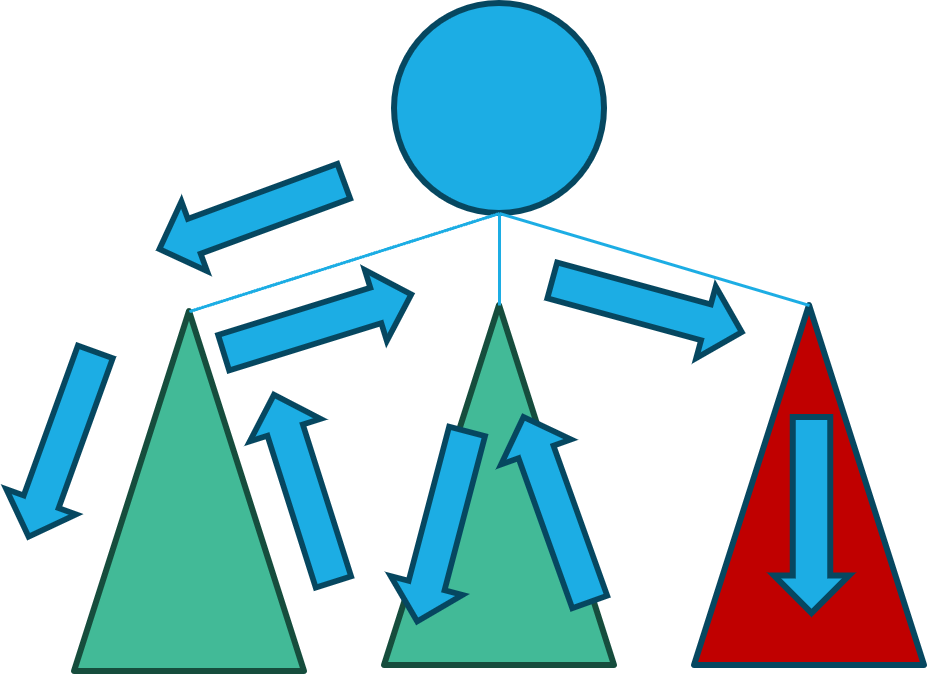
\includegraphics[width=0.9\linewidth]{./figure/fig1.png}
		\caption{\begin{CJK}{UTF8}{song}$\textrm{must}$~为真的点的结构\end{CJK}}
        \label{fig1a}%文中引用该图片代号
	\end{minipage}
	% \qquad
	%让图片换行，
	
	\begin{minipage}{\linewidth}
		\centering
		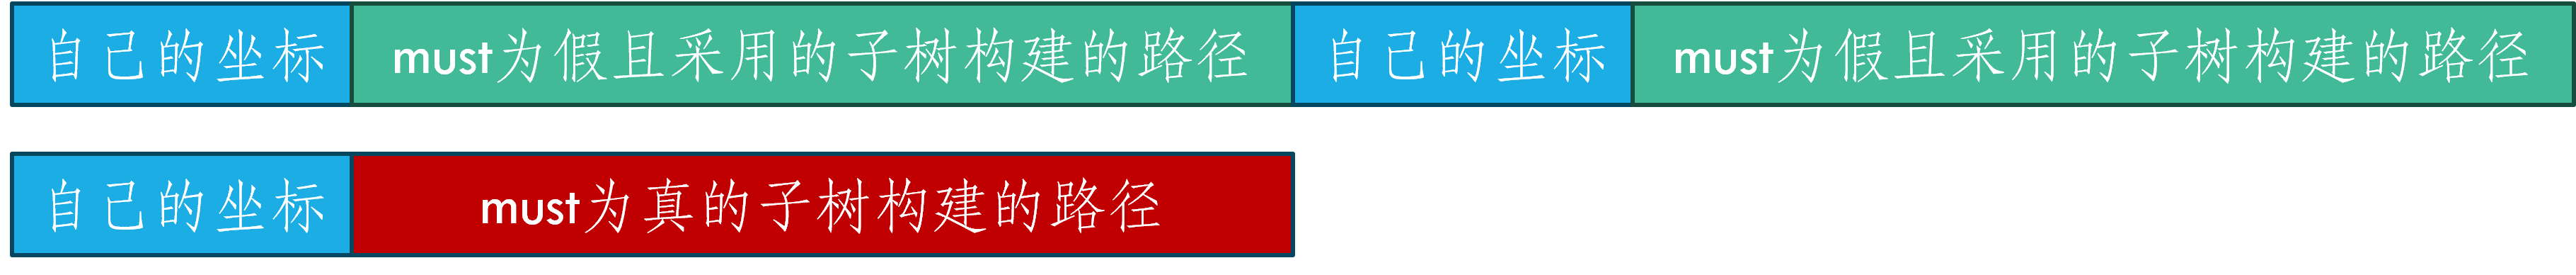
\includegraphics[width=0.9\linewidth]{./figure/fig2.png}
		\caption{\begin{CJK}{UTF8}{song}$\textrm{must}$~为真的点的路径构建顺序\end{CJK}}
		\label{fig2}%文中引用该图片代号
	\end{minipage}
% \centerline{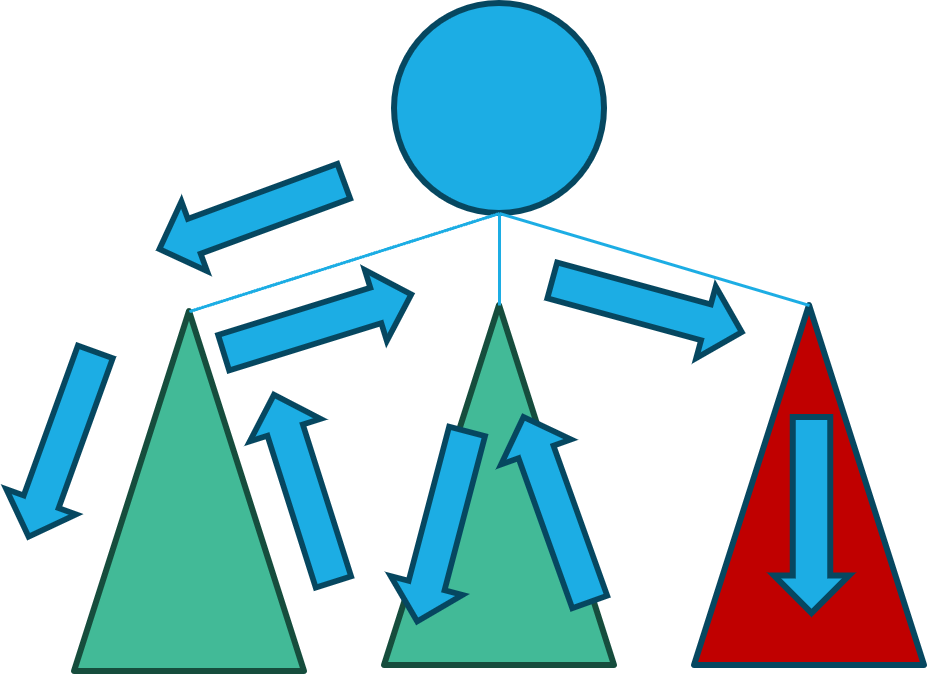
\includegraphics[width=3.15in,height=1.98in]{./figure/fig1.png}}
% \centerline{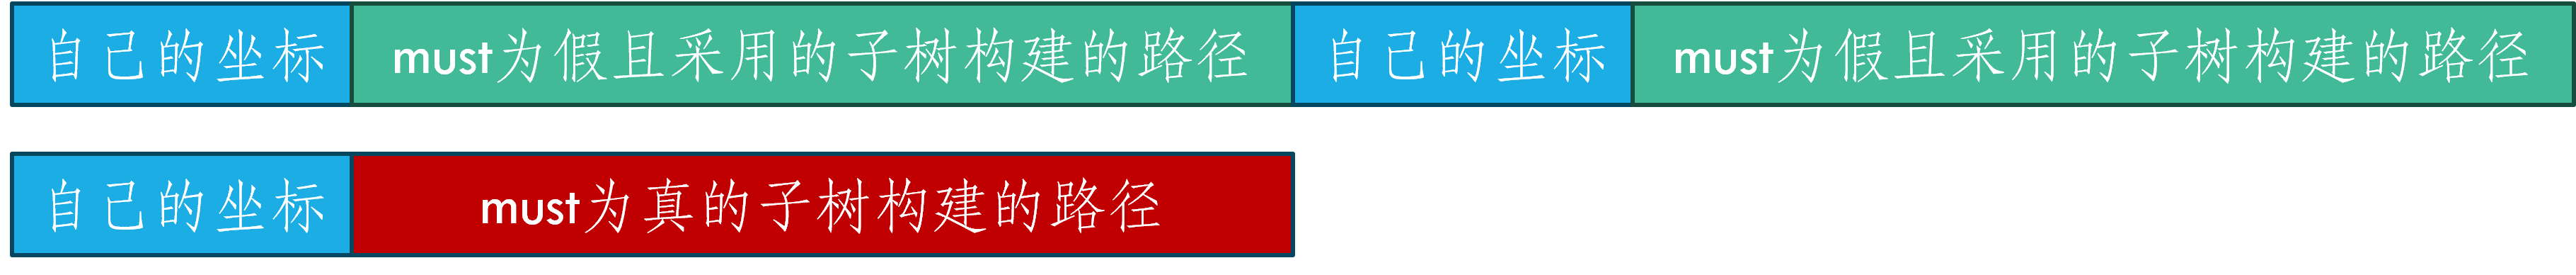
\includegraphics[width=3.15in,height=1.98in]{./figure/fig2.png}}
% 图X\quad  图片说明 *字体为小5号，图片应为黑白图，图中的子图要有子图说明*
% \label{fig2}
\end{figure}

% \begin{CJK*}{UTF8}{song}
% wssb

% \end{CJK*}

\begin{CJK*}{UTF8}{zhhei}\subsection{伪代码}\end{CJK*}

见附录~1.
% \end{CJK*}

% \begin{CJK*}{UTF8}{song}

{\begin{CJK*}{UTF8}{zhhei}\subsection{二级标题 *字体为5号黑体*标题2}\end{CJK*}}
\subsubsection{三级标题 *字体为5号宋体*标题3}
*正文部分, 字体为5号宋体* 正文文字

\textbf{正文文字要求语句通顺，无语法错误，结构合理，条理清楚，不影响审稿人、读者阅读理解全文内容。以下几类问题请作者们特别注意}：

1) 文章题目应明确反映文章的思想和方法；文字流畅，表述清楚；

2) 中文文字、英文表达无语法错误；

3) 公式中无符号、表达式的疏漏，没有同一个符号表示两种意思的情况；

4) 数学中使用的符号、函数名用斜体；

5) 使用的量符合法定计量单位标准；

6) 矢量为黑体，标量为白体；

7) 变量或表示变化的量用斜体；

8) 图表规范，量、线、序无误，位置正确(图表必须在正文中有所表述后出现，即{\ldots}如图1所示)(注意纵、横坐标应有坐标名称和刻度值)。

9) 列出的参考文献必须在文中按顺序引用，即参考文献顺序与引用顺序一致，各项信息齐全(格式见参考文献部分)；

10) 首次出现的缩写需写明全称，首次出现的符号需作出解释。

11) 图的图例说明、坐标说明全部用中文或量符号。

\textbf{12) 图应为矢量图。}

13) 表中表头文字采用中文。

14) 公式尺寸：

标准：10.5磅

下标/上标：5.8磅

次下标/上标：4.5磅

符号：16磅

次符号：10.5磅

15) 组合单位采用标准格式，如：``pJ/bit/m$^{4}$''应为 ``pJ/(bit$\cdot
$m$^{4})$''

{\begin{CJK*}{UTF8}{zhhei}\textbf{定理1}.\end{CJK*}}\quad ******. *定理内容.*

[``定义''、``假设''、``公理''、``引理''等的排版格式与此相同，详细定理证明、公式可放在附录中]

{\begin{CJK*}{UTF8}{song}证明\end{CJK*}}.\quad  *证明过程.* [``例 x''等的排版格式相同]

\rightline {证毕.}

\begin{figure}[htbp]
\centerline{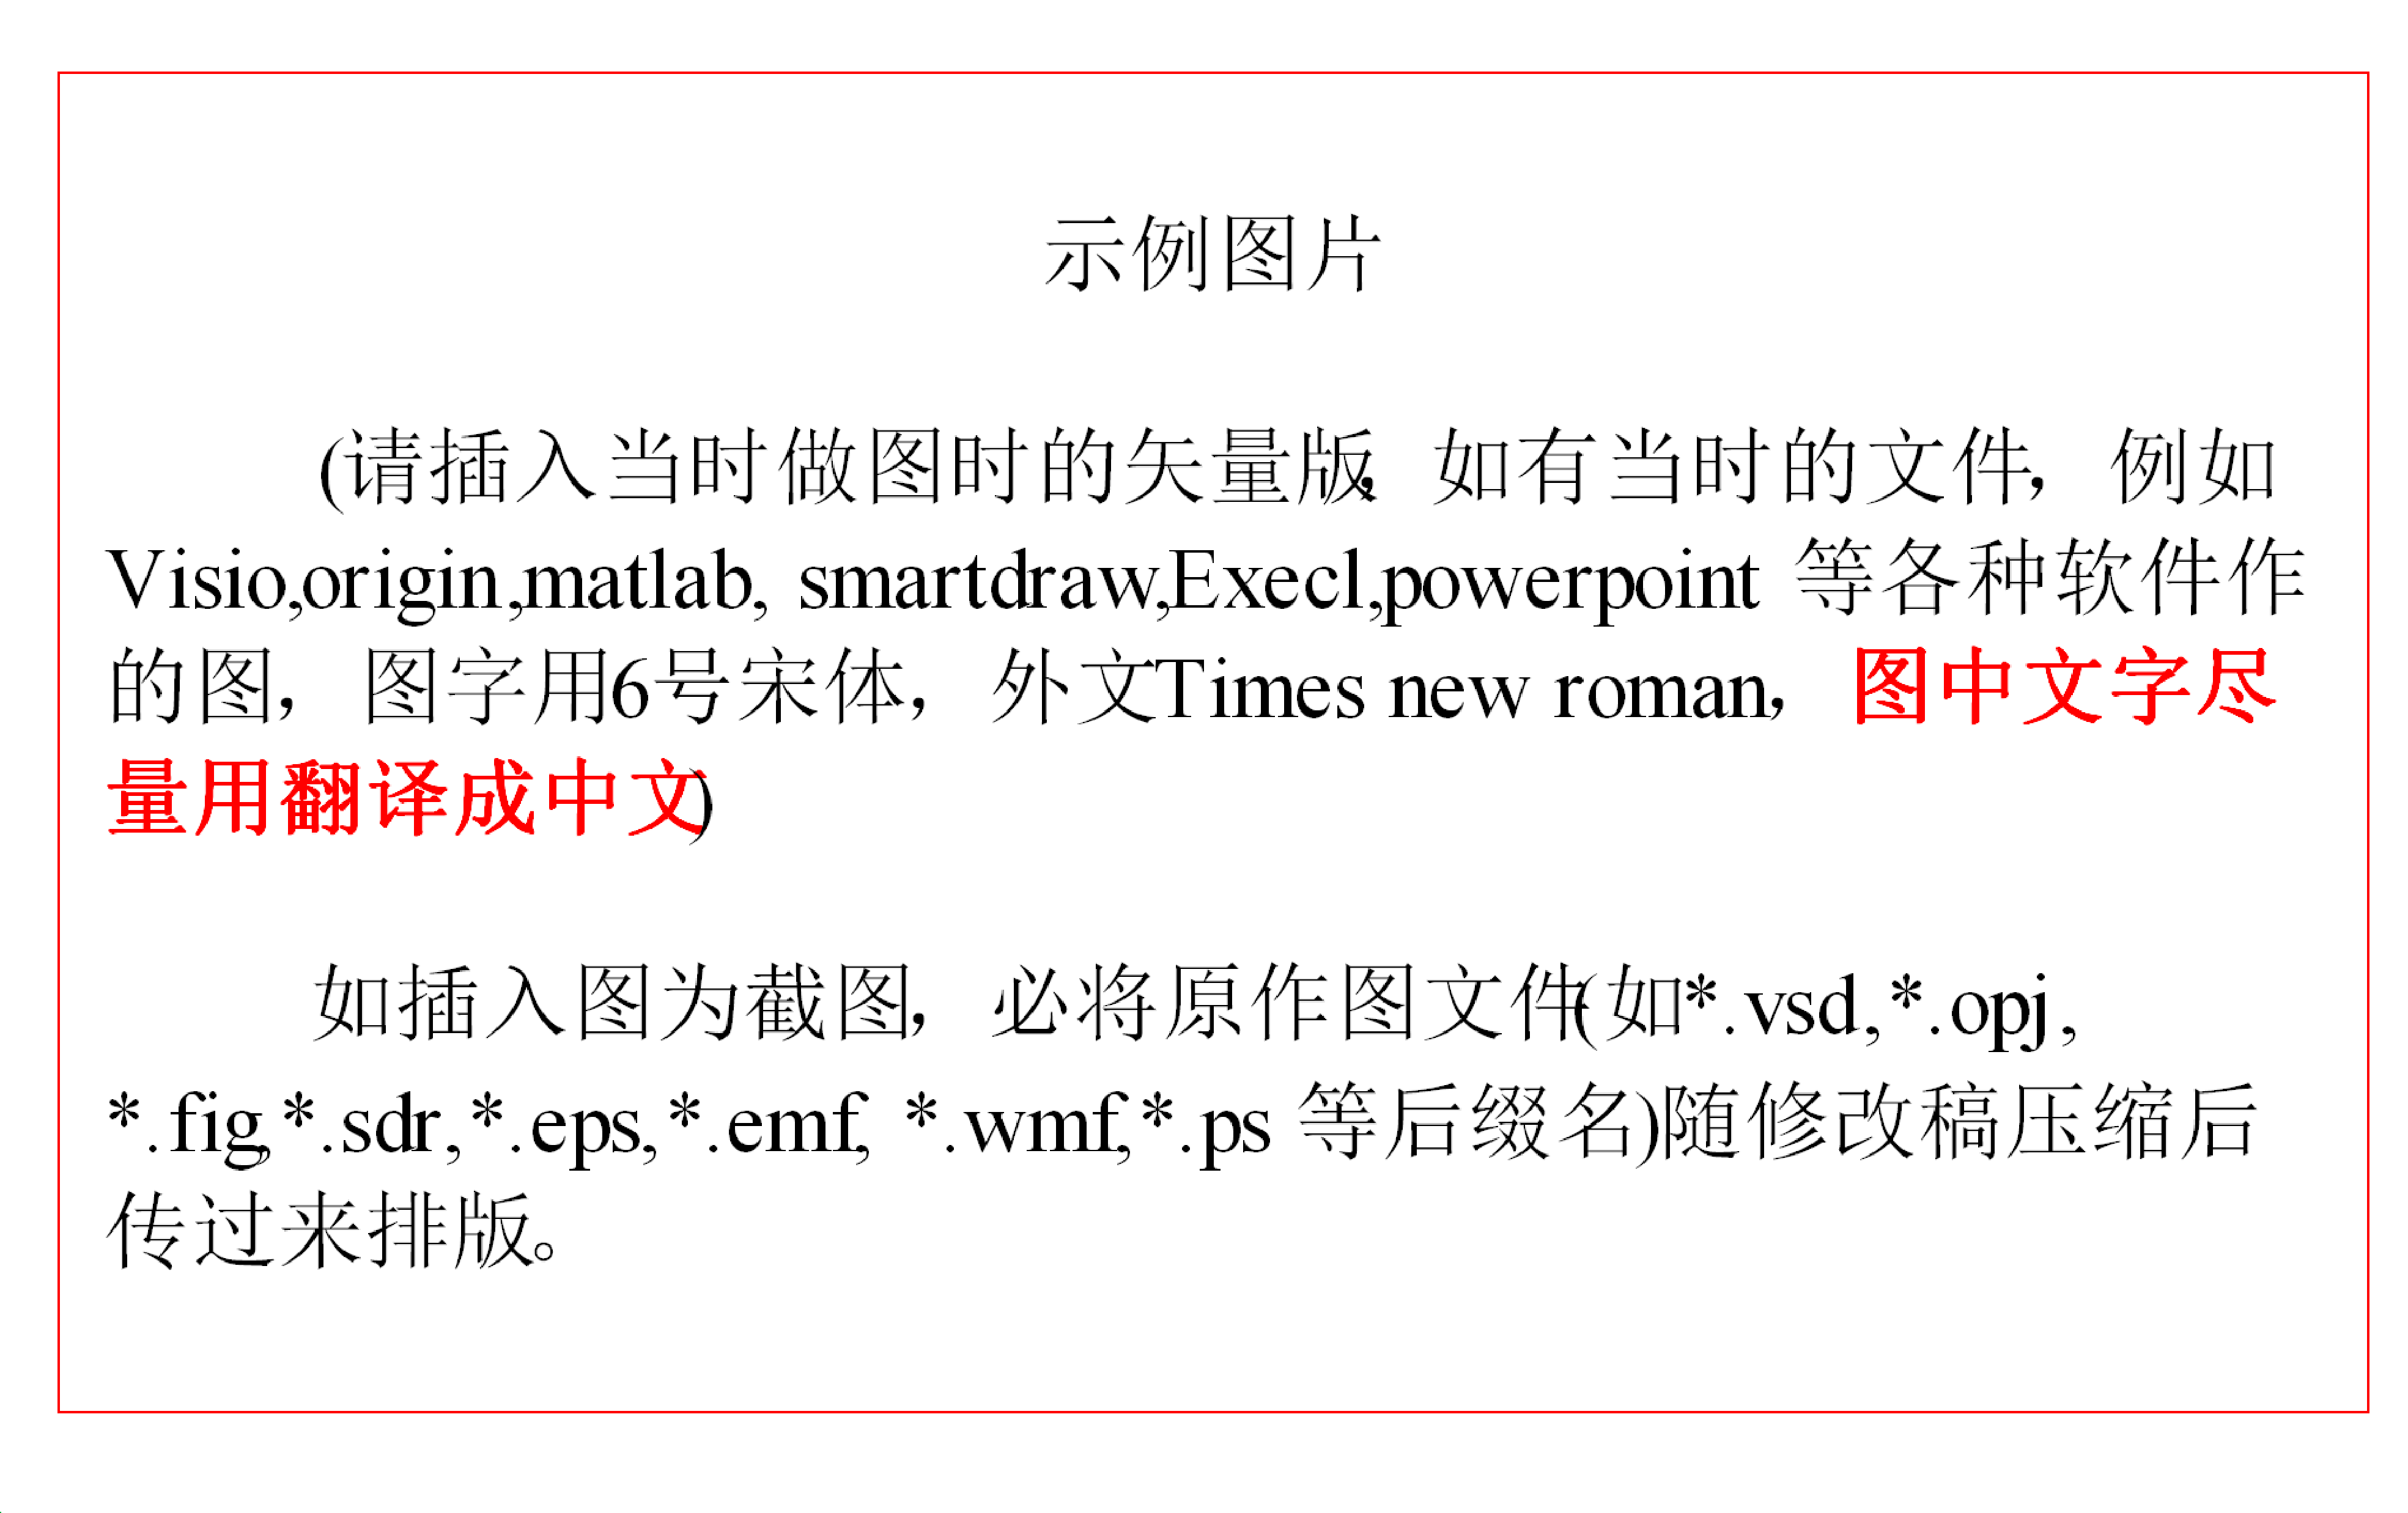
\includegraphics[width=3.15in,height=1.98in]{CJC1.pdf}}
图X\quad  图片说明 *字体为小5号，图片应为黑白图，图中的子图要有子图说明*
\label{CJC1}
\end{figure}

\begin{table}[htbp]
\centering {\begin{CJK*}{UTF8}{zhhei}表X\quad 表说明 *表说明采用黑体*\end{CJK*}}
\vspace {-2.5mm}
\begin{center}
\begin{tabular}{ll}
\toprule
*示例表格*&*第1行为表头,表头要有内容* \\
\hline
&
 \\
&
 \\
&
 \\
&
 \\
\bottomrule
\end{tabular}
\label{tab1}
\end{center}
\end{table}

\begin{CJK*}{UTF8}{zhhei}过程X.\end{CJK*}\quad 过程名称

{\zihao{5-}*《计算机学报》的方法过程描述字体为小5号宋体，IF、THEN等伪代码关键词全部用大写字母，变量和函数名称用斜体*}


\begin{CJK*}{UTF8}{zhhei}算法\textbf{Y}\end{CJK*}.\quad 算法名称.
\zihao{5-}{

\noindent 输入：{\ldots} {\ldots}

\noindent 输出：{\ldots} {\ldots}

*《计算机学报》的算法描述字体为小5号宋体, IF、THEN等伪代码关键词全部用大写字母，变量和函数名称用斜体*}

\vspace {3mm}
\zihao{5}{
\noindent \begin{CJK*}{UTF8}{zhhei}致\quad 谢\end{CJK*}\quad \begin{CJK*}{UTF8}{kai} *致谢内容.* 致谢\end{CJK*}}


\vspace {5mm}
\centerline
{\zihao{5}
\begin{CJK*}{UTF8}{zhhei}参~考~文~献\end{CJK*}}

\begin{thebibliography}{99}
\zihao{5-} \addtolength{\itemsep}{-1em}
\vspace {1.5mm}

\bibitem[1]{1}
网上的文献(举例：The Cooperative
Association for Internet Data Analysis(CAIDA),http://www.caida.org/data
2010,7,18) \textbf{*请采用脚注放于正文出现处，每页的脚注从1开始编序号*}
% \footnote{The Cooperative Association for Internet Data
% Analysis (CAIDA), http://www.caida.org/data 2010, 7, 18}

\bibitem[2]{2} 中文的参考文献需给出中英文对照。形式如[3]。

\bibitem[3]{3} Zhou Yong-Bin, Feng Deng-Guo. Design and analysis of cryptographic
protocols for RFID. Chinese Journal of Computers, 2006, 29(4): 581-589 (in
Chinese) \newline
(周永彬, 冯登国. RFID安全协议的设计与分析. 计算机学报, 2006, 29(4): 581-589)

\bibitem[4]{4} 期刊、会议、书籍名称不能用缩写。

\bibitem[5]{5} 作者(外国人姓在前，名在后可缩写, 后同).
题目(英文题目第一字母大写，其它均小写)：副标题(如果有). 刊名(全称), 年,
卷(期): 页码 \textbf{*期刊论文格式*}

\bibitem[6]{6}作者.
文章题目(英文题目第1字母大写，其它均小写)：副标题(如果有)//Proceedings of
the {\ldots} (会议名称). 会议召开城市, 会议召开城市所在国家, 年: 页码
\textbf{*会议论文集论文格式*}

\bibitem[7]{7}作者. 文章题目(英文题目第一字母大写, 其它均小写):
副标题(如果有)//编者. 文集标题. 出版地: 出版社, 出版年: 页码
\textbf{*文集格式*}

\bibitem[8]{8}作者. 书名: 副标题(如果有). 版次(初版不写). 出版社地点: 出版社,
出版年 \textbf{*书籍格式*}

\bibitem[9]{9}作者. 文章题目[博士学位论文/硕士学位论文]. 单位名称,单位地点, 年
\textbf{*学位论文格式*}

\bibitem[10]{10}作者. 文章题目(英文题目第一字母大写，其它均小写). 单位地点: 单位,
技术报告: 报告编号, 年 \textbf{*技术报告*}

\bibitem[11]{11}专利拥有人. 专利名称，专利授权国家，专利授权日期
\textbf{*技术专利*}
  \end{thebibliography}

\begin{strip}
\end{strip}

\noindent {\zihao{5}\bf{附录1}. 伪代码}


\begin{algorithm}
\caption{Maze Generation}
\begin{algorithmic}[1]
\Function{genMaze}{$n$}
    \State Initialize maze $M$ with walls
    \State Set entrance and exit on $M$ boundary
    \State $P \gets \emptyset$
    \State $r \gets \frac{n+1}{2}$
    \State \Call{getPath}{$P, 0,0,r-2,r-2$}
    \State \Call{destroyWall}{$P,M$}
    \State \Call{generateElements}{$M$}
    \State \Return $M$
\EndFunction

\Function{getPath}{$P,x_1,y_1,x_2,y_2$}
    \If{$x_1 = x_2$}
        \For{$i=y_1$ \textbf{to} $y_2-1$}
            \State $P \gets P \cup \{((x_1,i),(x_1,i+1))\}$
        \EndFor
        \State \Return
    \EndIf
    \If{$y_1 = y_2$}
        \For{$i=x_1$ \textbf{to} $x_2-1$}
            \State $P \gets P \cup \{((i,y_1),(i+1,y_1))\}$
        \EndFor
        \State \Return
    \EndIf
    \State Choose random $d_i \in [x_1,x_2-1]$, $d_j \in [y_1,y_2-1]$
    \State Open doors around $(d_i,d_j)$, add to $P$
    \State \Call{getPath}{$P,x_1,y_1,d_i,d_j$}
    \State \Call{getPath}{$P,d_i+1,y_1,x_2,d_j$}
    \State \Call{getPath}{$P,d_i+1,d_j+1,x_2,y_2$}
    \State \Call{getPath}{$P,x_1,d_j+1,d_i,y_2$}
\EndFunction

\Function{destroyWall}{$P,M$}
    \ForAll{$e=((x_1,y_1),(x_2,y_2)) \in P$}
        \If{$x_1 = x_2$}
            \State Remove vertical wall between points in $M$
        \Else
            \State Remove horizontal wall between points in $M$
        \EndIf
    \EndFor
\EndFunction

\Function{generateElements}{$M$}
    \ForAll{empty cell $c$}
        \State Place boss, locker, trap, resource with given probabilities
    \EndFor
\EndFunction
\end{algorithmic}
\end{algorithm}

% \begin{strip}
% \end{strip}

% \noindent {\zihao{5}\bf{附录X}.}
% \zihao{5}
% \noindent \textbf{Background}

% \zihao{5-}\setlength\parindent{2em}
% *\textbf{附录内容}置于此处，字体为小5号宋体。附录内容包括：\textbf{详细的定理证明、公式推导、原始数据}等*


% \begin{biography}[yourphotofilename.jpg]
% \noindent
% \textbf{First A. Author}\ \ *计算机学报第1作者提供照片电子图片，尺寸为1寸。英文作者介绍内容包括：出生年,学位(或目前学历),职称,主要研究领域(\textbf{与中文作者介绍中的研究方向一致}).*
% *字体为小5号Times New Roman*

% \end{biography}

% \begin{biography}[yourphotofilename.jpg]
% \noindent
% \textbf{Second B. Author} *英文作者介绍内容包括：出生年,学位(或目前学历),职称,主要研究领域(\textbf{与中文作者介绍中的研究方向一致})。*
% *字体为小5号Times New Roman*
% \end{biography}
% \begin{strip}
% \end{strip}
% \zihao{5}
% \noindent \textbf{Background}

% \zihao{5-}{
% \setlength\parindent{2em}
% *论文背景介绍为\textbf{英文}，字体为小5号Times New Roman体*

% 论文后面为400单词左右的英文背景介绍。介绍的内容包括：

% 本文研究的问题属于哪一个领域的什么问题。该类问题目前国际上解决到什么程度。

% 本文将问题解决到什么程度。

% 课题所属的项目。

% 项目的意义。

% 本研究群体以往在这个方向上的研究成果。

% 本文的成果是解决大课题中的哪一部分，如果涉及863$\backslash
% $973以及其项目、基金、研究计划，注意这些项目的英文名称应书写正确。}

\end{CJK*}
\end{document}


